% ==========================================
% SEÇÃO 5: IMPLEMENTAÇÃO E COMPUTAÇÃO GRÁFICA AVANÇADA
% ==========================================
\section[Implementação]{Implementação e Computação Gráfica Avançada}

\begin{frame}{Cores em OpenGL e o Canal Alpha}
    \begin{columns}[T]
        \begin{column}{0.55\textwidth}
            \textbf{Alocação de Memória (VRAM):}
            \begin{itemize}
                \item Em arquiteturas de 32 bits, cada pixel é um array contíguo de 4 bytes na GPU: \texttt{[R, G, B, A]}.
                \item O canal \textbf{Alpha} mapeia a opacidade escalar como um ponto flutuante de \texttt{0.0} (transparente) a \texttt{1.0} (opaco).
            \end{itemize}
            
                \vspace{0.2cm}
            
                \textbf{O Algoritmo de Blending:}
            \begin{itemize}
                \item Para renderizar transparência, o hardware mistura a cor do novo fragmento (\textit{Source}) com a cor já gravada no Framebuffer (\textit{Destination}).
            \end{itemize}
        \end{column}
        
        \begin{column}{0.45\textwidth}
            \begin{figure}
                \centering
                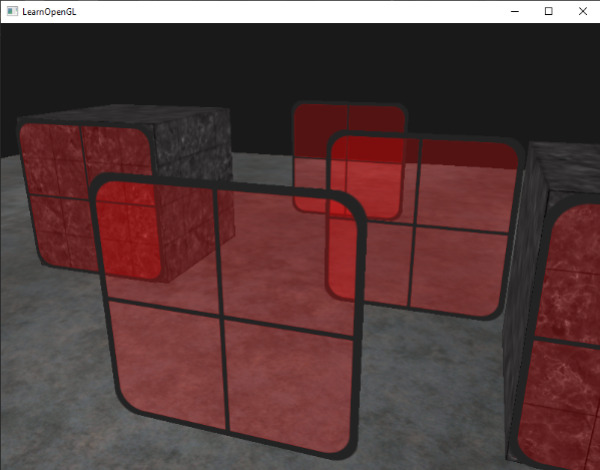
\includegraphics[width=0.9\textwidth]{images/mecanismo_blending.jpg}
                \caption{Operação de Alpha Blending diretamente nos registradores do Framebuffer.}
            \end{figure}
        \end{column}
    \end{columns}

    \note{
        \begin{columns}[T]
            \begin{column}{0.49\textwidth}
                \scriptsize
                \textbf{Gargalo do Z-Buffer:}
                \begin{itemize}
                    \setlength{\itemsep}{1pt}
                    \item \textbf{A Ordem de Renderização:} Objetos opacos podem ser desenhados em qualquer ordem porque o teste de profundidade (Z-buffer) descarta pixels tapados. Objetos transparentes que usam blending quebram essa lógica. A equação matemática não é comutativa; se o programador desenhar o fundo após o objeto transparente, o cálculo falha.
                \end{itemize}
            \end{column}

            \begin{column}{0.49\textwidth}    
                \scriptsize
                \textbf{Solução em Software:}
                \begin{itemize}
                    \setlength{\itemsep}{1pt}
                    \item \textbf{Ordenação de Polígonos:} Engines de jogos precisam ordenar todas as geometrias translúcidas da cena com base na distância da câmera (do mais distante para o mais próximo) a cada frame antes de enviar os dados de vértice para os Draw Calls da API gráfica.
                \end{itemize}
            \end{column}
        \end{columns}   
    }
\end{frame}

\begin{frame}{Técnicas Avançadas de Realismo Cromático}
    \begin{columns}[T]
        \begin{column}{0.5\textwidth}
            \textbf{Lightmaps (Iluminação Pré-Calculada):}
            \begin{itemize}
                \item Calcular equações de raio (\textit{Ray Tracing}) em tempo real a 60 FPS é computacionalmente proibitivo para hardware comum.
            \end{itemize}
            
            \vspace{0.2cm}
            
            \textbf{Sub-Surface Scattering (SSS):}
            \begin{itemize}
                \item Algoritmo que simula a física de materiais translúcidos (pele, cera, folhas).
            \end{itemize}
        \end{column}
        
        \begin{column}{0.5\textwidth}
            \begin{figure}
                \centering
                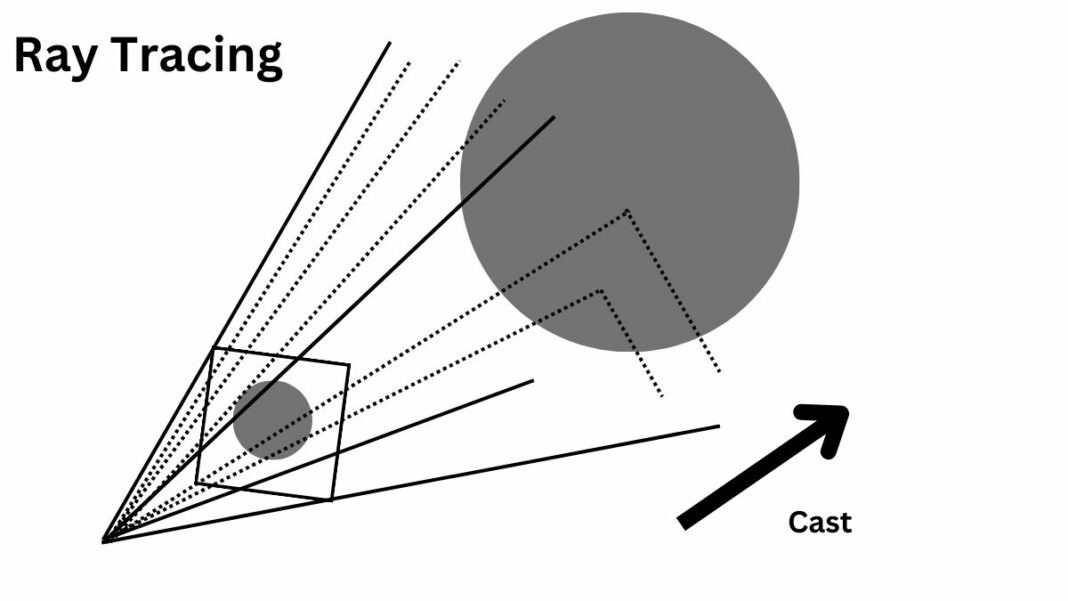
\includegraphics[width=0.9\textwidth]{images/subsurface_scattering_demo.jpg}
                \caption{Comportamento físico dos vetores de luz na técnica de SSS.}
            \end{figure}
        \end{column}
    \end{columns}

    \note{
        \begin{columns}[T]
            \begin{column}{0.49\textwidth}
                \scriptsize
                \textbf{Otimização de Textura:}
                \begin{itemize}
                    \setlength{\itemsep}{1pt}
                    \item \textbf{Custo de Memória:} O uso de Lightmaps zera o custo de processamento de shaders de iluminação dinâmica na CPU/GPU durante a execução do software. O trade-off é estritamente o consumo de VRAM, já que o jogo precisa carregar texturas adicionais de alta resolução contendo apenas o mapa de sombras mapeado na malha.
                \end{itemize}

                \textbf{Sub-Surface Scattering (SSS):}
                \begin{itemize}
                    \item Simula a física de materiais translúcidos (pele, cera, folhas).
                    \item Os fótons não ricocheteiam na superfície; eles penetram o material, sofrem desvios internos e saem em outra coordenada.
                \end{itemize}
            \end{column}

            \begin{column}{0.49\textwidth}    
                \scriptsize
                \textbf{Física de Shaders (SSS):}
                \begin{itemize}
                    \setlength{\itemsep}{1pt}
                    \item \textbf{O Efeito Plástico:} Sem o algoritmo de SSS, a iluminação aproximada clássica (Lambert/Phong) trata a geometria como opaca pura. Em bordas finas retroiluminadas (como uma orelha contra o sol), a ausência do espalhamento interno faz a pele parecer plástico escuro e sem vida, destruindo o fotorrealismo.
                \end{itemize}

                \textbf{Lightmaps (Iluminação Pré-Calculada):}
                \begin{itemize}
                    \item \textbf{Solução:} As sombras e rebatimentos de luz estáticos são processados na compilação (\textit{Baking}) e salvos como texturas normais injetadas no segundo canal de UV da malha.
                \end{itemize}
            \end{column}
        \end{columns}   
    }

\end{frame}





\begin{frame}{O Algoritmo de Dithering e a Ilusão Cromática}
    \begin{columns}[T]
        \begin{column}{0.55\textwidth}
            \textbf{Quantização e Redução de Cores:}
            \begin{itemize}
                \item Técnica matemática para simular maior profundidade de cor (bits por pixel) em hardwares com paletas severamente limitadas.
                \item Utiliza padrões geométricos de pixels ou difusão de erro para enganar a percepção humana.
            \end{itemize}
            
            \vspace{0.2cm}
            
            \textbf{O Papel do Hardware Analógico (CRT):}
            \begin{itemize}
                \item A imperfeição física dos monitores CRT atuava como um filtro passa-baixa natural, fundindo os pixels em degradês suaves.
            \end{itemize}
        \end{column}
        
        \begin{column}{0.45\textwidth}
            \begin{figure}
                \centering
                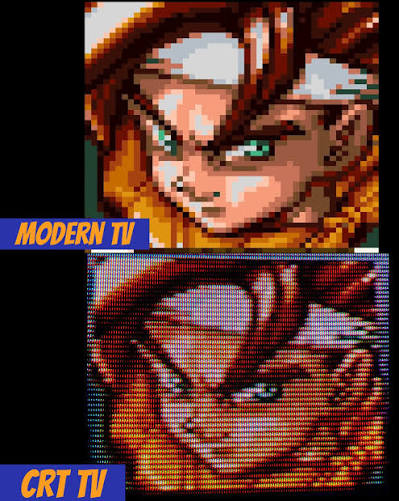
\includegraphics[width=0.7\textwidth]{images/chrono_trigger.png}
                \caption{Fusão óptica de pseudo-cores através de entrelaçamento de pixels em malhas CRT.}
            \end{figure}
        \end{column}
    \end{columns}

    \note{
        \begin{columns}[T]
            \begin{column}{0.49\textwidth}
                \scriptsize
                \textbf{Difusão de Erro (Floyd-Steinberg):}
                \begin{itemize}
                    \setlength{\itemsep}{1pt}
                    \item \textbf{A Matemática:} O algoritmo calcula a diferença entre a cor original do pixel e a cor mais próxima disponível na paleta. Esse erro residual é distribuído/difundido para os pixels vizinhos ainda não processados usando uma matriz de pesos.
                \end{itemize}
            \end{column}

            \begin{column}{0.49\textwidth}    
                \scriptsize
                \textbf{Anacronismo Digital (LCD/OLED):}
                \begin{itemize}
                    \setlength{\itemsep}{1pt}
                    \item \textbf{Quebra da Ilusão:} Telas modernas exibem pixels estritos com matrizes nítidas e sem vazamento de luz. Sem o desfoque do CRT, os padrões de dithering tornam-se artefatos de ruído visíveis. Engines modernas aplicam filtros de interpolação para restaurar o efeito pretendido originalmente.
                \end{itemize}
            \end{column}
        \end{columns}   
    }
\end{frame}


